%************************************************
\chapter{Introduction}\label{ch:introduction}
%************************************************
\section{Spintronics and the limitations of every day electronics}
In today's society electronic devices are heavily incorporated in everyone's daily life. The everlasting desire to make our computers run faster, necessarily leads to smaller and smaller electric components. Where in the early 70s a single computer chip could host up to a few thousands of transistors, today the number approaches tens to hundreds of billions and soon will reach a fundamental limit \cite{mccleanreport}. 

At the heart of electronic devices are electronic circuits that control the charge of electrons. Besides charge, electrons however poses two spin states that can be named "up" and "down", a degree of freedom that can be utilized in both data storage and processing. The giant magneto-resistance effect \cite{binasch_enhanced_1989, baibich_giant_1988} for example has made a tremendous impact on data storage technologies \cite{puebla_spintronic_2020}. 

Unfortunately these improvements in computer chips and data storage has lead to an increase in energy consumption. Predictions say the total electricity demand of information and communication technology will be 20.9\% of the total world's electricity demand \cite{jones_how_2018} by 2030. 

Spin-based electronics or "spintronics" as it is often referred to, has become an active field of research. Compared with charge-based devices, spin-based devices could in principle have higher density, lower energy cost, and faster operating speed \cite{pu_chapter_2020, liu_chapter_2020, book_recent_advancements}. Despite active research, many open questions remain about the electron spin dynamics. These include among others understanding the effects of spin-orbit coupling, spin-valley coupling, and spin-photon interaction \cite{liu_chapter_2020, hellman_interface-induced_2017}. 

% Electronics all revolve around the control of the charge of electrons. These electrons however also posses a magnetic moment called spin. The utilization of this spin degree of freedom, leads to the an emerging field called spintronics.

% Spintronics has many advantages over traditional electronics, such as no volatility, high data processing speed, low energy consumption, and high integration density. \cite{book_recent_advancements}


% %%%%
% Spin-based phenomena are rich in fundamental physics and important to information technology. Many aspects of electron spin dynamics remain open questions, including spinorbital coupling, spinphoton interaction, spin ordering at low dimensions, and spin- wave transmission to name a few. Since the discovery of the giant magnetoresistance effect (GMR), celebrated by the 2007 Nobel Prize in Physics, spin-based electronics—or “spintronics” as it quickly became known—has developed into an interdisciplinary field dedicated to the study of spin-based effects rather than purely charge-based physical phenomena previously associated with electronic systems (Fig. 1.1). This eventually led to a revolutionary impact on device concepts, particularly in data storage technologies where the introduction of spintronic technologies enabled a rapid increase in the capacity of hard drives.
% \cite{liu_chapter_2020}

% Spintronics has many advantages over traditional electronics, such as no volatility, high data processing speed, low energy consumption, and high integration density. Therefore, spintronics, which utilizes spin instead of charge as the carrier for information transportation and processing, can be seen as one of the most promising ways to implement high-speed and low-energy electronic devices. However, in the process of developing spintronic devices, we have also encountered many bottlenecks, including spin-polarized carrier generation and injection, long-range spin-polarization transport, and spin manipulation and detection. To overcome these problems, various types of spintronic materials have been proposed
% \cite{book_recent_advancements}

% Electron spin has two degenerate states, namely “up” and “down,” in the contrary with the electron charge that has a fixed value. In information technology the two states of electron spin can represent “0” and “1” states for data storage, and the transition between the two states can be used for logic operation. Down to atomic level B1 nm, the spin coupling energy between nearby electrons could be orders of magnitude smaller than the coulomb interaction. Compared with charge-based devices, spin-based devices could in principle have higher density, lower energy cost, and faster speed.
% The main goal of spintronics is to utilize spin as basic unit in logic to build electronic devices for information storage and processing. To achieve that, four fundamental operations on spins are generally required: spin generation, spin detection, spin manipulation, and spin transport, as sketched in Fig. 5.1. Among the four operations the spin generation is usually the first step since there is always required to generate enough spins for further operation, from the device point of view a spintronic device needs to be driven by a spin source or spin current; spin detection is used to determine the orientation of spins for information read-out; spin manipulation and spin transport are usually used for information processing and communication, respectively [1].
% Charge-spin conversion in 2D systems 127
%   Figure 5.1
% Basic spin operations: spin generation, spin detection, spin manipulation, and spin transport.
% These four operations on spins have been realized in practice by different methods, including electrical, optical, mechanical, and thermal. Although in principle a spintronic device can be operated by either one or combination of these methods, the electrical control that has been well developed in modern electronics is the dominant method for spintronic devices, which is also the main focus of this chapter. From the material point of view the four spin operations have been achieved in conventional bulk materials. However, the fast development of modern spintronics demands new devices with much better performance, which become more and more challenging for bulk materials. More and more attentions have been attracted on the spin operations in 2D systems to design new devices with higher density, lower energy cost, and faster speed.
% Although spin-based devices have advantages over charge-based devices for many aspects, the spin generation and spin detection are still the major challenges for the development of modern spintronics. In the contrary with charge, spin is not a conserved number. Given the fact that the spin lifetime is generally very short (picosecond or less in metals and nanosecond in semiconductors), spin information can be easily lost due to spin-flip or spin-dephasing. Unlike various electrical sources and detections for charge- based devices, to date suitable spin sources and sensitive spin detection are still lacking in most of cases.
% \cite{pu_chapter_2020}
% %%%%
% In todays society electronic devices are heavily incorporated in everyone's daily life. What is responsible for the ever increasing power of these devices is our better control of the electric charge. The transistor for example controls the flow of charge (turning it "on" and "off") by setting a gate voltage. The flow of charge however necessarily produces heat. Although a single unit in a microprocessor does not produce too much heat, fifty billion transistors.. It is predicted that in mere decades data centers and servers will demand roughly 50\% of the worlds energy demand just to cool the computers. 

% The ever increasing industrial techniques make it possible to push electronics to their physical limit. As of writing ASML holds the record for most number of transistors built on a chip. Where in the early 70s a single computer chip could host up to a few thousands of transistors, it now approaches fifty billion. The physical limit ranges from the diffraction limit, which is overcome by using a laser with higher frequency, to the atomic limit. The average size of a transistor is ..., whereas the size of a bit in a magnetic hard drive is about. Another unwanted byproducts of each technological leap is the production of heat. 

% Today's electronics revolves around the control of the electron's charge. By moving these charges around in electronic circuits, complex calculations can be made in mobile phones, computers,... As technology makes new advancements every year, we see that the size of electronic circuits gets smaller and smaller. A popular ``law'' used to show this advancement is named after Moore. It roughy states that the number of transistors that can be put unto a single chip doubles every two years. Where in the early 70s a single computer chip could host up to a few thousands of transistors, today the number approaches fifty billion.  

% Another commercial area where spintronics could make a leapthrough is storage devices. Until a few years ago a magnetic hard-drive was the best storage medium. 

% Electronics all revolve around the control of the charge of electrons. These electrons however also posses a magnetic moment called spin. The utilization of this spin degree of freedom, leads to the an emerging field called spintronics. Here the electrical control of spin-currents and magnetization is studied and it is believed that spintronic devices could potentially lead to more efficient data storage and faster reading/writing speeds than in conventional electronics. One of the main goals in this field is to discover how to efficiently convert charge into spin currents in devices without any magnetic contacts. 


% \section{Two dimensions}
% Many properties of a crystal are defined by its symmetries. At the surface of a three-dimensional crystal one of the translational symmetries is broken, leading to so-called surface states. These surface states are two-dimensional in nature and are in general very distinct from the states in the bulk. Similarly, electrons can also be confined between the interface of two crystals leading to similar two-dimensional states. Two dimensional systems have electronic and transport properties that are not found in three-dimensional crystals making them attractive alternatives to silicon-based electronics. Moreover, if the systems lack inversion symmetry it gives rise to Rashba spin-orbit coupling (more details below) which is a focus of the study in this Thesis. 

% After the discovery of the first real two-dimensional crystal --- graphene --- many others were found. 
\subsection{Spintronics in ferro- and antiferromagnets}
Ferromagnetic spintronics has greatly contributed to microelectronic technology in the last few decades \cite{bader_spintronics_2010, sinova_new_2012, bhatti_spintronics_2017}. One of the practical results was the development of magnetic memories with purely electronic write-in and read-out processes as an alternative to existing solid state drive technologies \cite{kent_new_2015, sato_two-terminal_2018}.

Ferromagnetic thin films have already entered commercial use in hard drives, magnetic field and rotation angle sensors and in similar devices \cite{Parkin2003,Jogschies2015,Novoselov2019}, while keeping high promises for technologically competitive ultrafast memory elements \cite{Lau2016} and neuromorphic chips \cite{Fukami2016}. 

It is widely known that spin-orbit interaction provides an efficient way to couple electronic and magnetic degrees of freedom. It is, therefore, no wonder that the largest torque on magnetization, which is also referred to as the spin-orbit torque, emerges in magnetic systems with strong spin-orbit interaction \cite{miron_current-driven_2010,haney_current_2013} as has been long anticipated \cite{dyakonov_current-induced_1971}. 

The spin-orbit coupling may be enhanced by confinement potentials in effectively two-dimensional systems consisting of conducting and magnetic layers. The in-plane current may efficiently drive domain walls or switch magnetic orientation in such structures with the help of spin-orbit torque \cite{awschalom2009trend,manchon_theory_2008,garate_influence_2009,manchon2009theory}, which is present even for uniform magnetization, or with the help of spin-transfer torque, which requires the presence of magnetization gradient (due to e.\,g. domain wall) \cite{slonczewski_current-driven_1996,berger_emission_1996, ralph_spin_2008, stiles_anatomy_2002}. 

On the other hand, antiferromagnets have received a great deal of attention due to their high temperature magnetic order in a large variety of materials. The study of antiferromagnets have uncovered many interesting properties. For example, the antiferromagnet has zero magnetic moment, is
insensitive to external fields and contains no internal stray fields.
Furthermore, ultrafast switching of the antiferromagnetic order has been observed \cite{gomonay_high_2016, olejnik_terahertz_2018, jungwirth_multiple_2018, macdonald_antiferromagnetic_2011,gomonay_spintronics_2014,zelezny_relativistic_2014}. In
spintronic devices these properties translate to storing magnetic data at high densities, fast
reading and writing, and, in addition to low energy consumption, make the antiferromagnet an ideal
candidate for further study.

An increasing demand for ever higher performance computation and ever faster big data analytics has therefore sparked the interest to antiferromagnetic spintronics \cite{macdonald_antiferromagnetic_2011, gomonay_spintronics_2014, wadley_electrical_2016, jungwirth_antiferromagnetic_2016, baltz_antiferromagnetic_2018, jungwirth_multiple_2018, jungfleisch_perspectives_2018}, i.\,e. to the usage of the much more subtle antiferromagnetic order parameter to store and process information. This idea is driven primarily by the expectation that antiferromagnetic materials may naturally allow for up to THz operation frequencies \cite{gomonay_high_2016, olejnik_terahertz_2018, jungwirth_multiple_2018, macdonald_antiferromagnetic_2011,gomonay_spintronics_2014,zelezny_relativistic_2014} in sharp contrast to ferromagnets whose current-induced magnetization dynamics is fundamentally limited to GHz frequency range. 
  
% The best efficiency in electric switching of magnetic domains is achieved in systems involving materials with at least partial spin-momentum locking \cite{fina_electric_2017} due to sufficiently strong spin-orbit interaction. The latter is responsible for the so-called spin-orbit torques on magnetization that are caused by sizable non-equilibrium spin polarization induced by an electron flow \cite{brataas_current-induced_2012, Hals2013, zelezny_relativistic_2014, freimuth_spin-orbit_2014, ghosh_spin-orbit_2017, smejkal_electric_2017, zelezny_spin_2018, zhou_strong_2018, manchon_current-induced_2019, moriyama_spin-orbit-torque_2018, li_manipulation_2019, chen_electric_2019, zhou_large_2019, zhou_fieldlike_2019, bodnar_writing_2018}.  

Recently, spin-orbit-torque-driven electric switching of the N\'eel vector orientation has been predicted \cite{zelezny_relativistic_2014} and discovered in non-centrosymmetric crystals such as CuMnAs \cite{wadley_electrical_2016, fina_electric_2017, zelezny_spin_2018, saidl_optical_2017} and Mn$_2$Au \cite{barthem_revealing_2013, jourdan_epitaxial_2015, bhattacharjee_neel_2018}. Even though many antiferromagnetic compounds are electric insulators \cite{pandey_doping_2017}, which limits the range of their potential applications, e.g., for spin injection \cite{tshitoyan_electrical_2015}, the materials like CuMnAs and Mn$_2$Au possess  semi-metal and metal properties, inheriting strong spin-orbit coupling and sufficiently high conductivity. These materials also give rise to collective mode excitations in THz range \cite{bhattacharjee_neel_2018}. 

Despite a lack of clarity concerning the microscopic mechanisms of the N\'eel vector switching, these experiments have been widely regarded as a breakthrough in the emerging field of THz spintronics \cite{bhattacharjee_neel_2018, gomonay_high_2016, olejnik_terahertz_2018, jungwirth_multiple_2018, wadley_electrical_2016, jungwirth_antiferromagnetic_2016, baltz_antiferromagnetic_2018, jungfleisch_perspectives_2018}. It has been suggested that current-induced N\'eel vector dynamics in an AFM is driven primarily by the so-called N\'eel spin-orbit torques \cite{brataas_current-induced_2012, Hals2013, zelezny_relativistic_2014, freimuth_spin-orbit_2014, ghosh_spin-orbit_2017, smejkal_electric_2017, zelezny_spin_2018, zhou_strong_2018, manchon_current-induced_2019, moriyama_spin-orbit-torque_2018, li_manipulation_2019, chen_electric_2019, zhou_fieldlike_2019, zhou_large_2019, bodnar_writing_2018}. The N\'eel spin-orbit torque originates in a non-equilibrium staggered polarization of conduction electrons on AFM sublattices \cite{zelezny_relativistic_2014, smejkal_electric_2017, zelezny_spin_2018, manchon_current-induced_2019}. Characteristic magnitude of the non-equilibrium staggered polarization and its relevance for the experiments with CuMnAs and Mn$_2$Au remain, however, debated. 
% Despite their ubiquitousness, AFM materials have, however, avoided much attention from technology due to an apparent lack of control over the AFM order parameter -- the N\'eel vector. Switching the N\'eel vector orientation by short electric pulses has been put forward only recently as the basis for AFM spintronics \cite{macdonald_antiferromagnetic_2011,gomonay_spintronics_2014,zelezny_relativistic_2014}. 
% The proposed phenomenon has been soon observed in non-centrosymmetric crystals such as CuMnAs \cite{wadley_electrical_2016, fina_electric_2017, zelezny_spin_2018, saidl_optical_2017} and Mn$_2$Au \cite{barthem_revealing_2013, jourdan_epitaxial_2015, bhattacharjee_neel_2018}. It should be noted that in most cases AFMs are characterized by insulating type behavior \cite{pandey_doping_2017}, limiting the range of their potential applications, e.g., for spin injection \cite{tshitoyan_electrical_2015}. Interestingly, antiferromagnetic Mn$_2$Au possesses a typical metal properties, inheriting strong spin-orbit coupling and high conductivity, and is characterized by collective modes excitations in THz range \cite{bhattacharjee_neel_2018}.

%The electronic control of ferromagnetic domains is described by spin-torques. The misalignment of the spins of conducting electrons and the magnetic moment of localized electrons lead to so-called spin-torques. These torques that are induced by electric currents are the key concept in spintronics and can be used to the reverse the direction of magnetization and to drive magnetic domain walls. We distinguish two types of current-induced spin torque: spin-transfer torque and spin-orbit torque. Spin-transfer torques generally vanish in uniform magnets and are proportional to gradients in magnetization. These torques arise from the transfer of spin angular momentum from a spin-current to the spin degree of freedom of a ferromagnetic region.  On the other hand, the spin-orbit torque is in general proportional to magnetization (and can therefore be found in uniform magnets) and is mediated by spin-orbit interactions. 

% This last type of torque was first found in systems with a heavy metal layer [9], where the spin Hall
% effect (SHE) [10–13] plays an important role [? ]. Due to its the strong thickness dependence, the SOT
% produced by the SHE is limited to bulk materials [? ]. Later, more efficient charge-spin conversion was
% found in heavy metal interfaces that support Rashba spin-orbit interaction [10, 14–16].
% Recently spin- orbit torques were observed in bilayers consisting of a ferromagnet (FM) and a 3D
% topological insulator (TI) [17, 18]. The 3D TI was proposed as a 3D extension of the Quantum Spin
% Hall Insulator [19–22]. Its surface state consists of electrons that are described by a 2D Dirac
% equation and are called Dirac fermions. Because the kinetic energy of the Dirac fermions is essentially
% only spin-orbit interaction, spin and momentum are highly correlated. It is believed that this
% spin-momentum locking – together with the topological properties of the TI – could lead to even
% greater charge-spin conversion [23]. 

% \subsection{Spintronics in antiferromagnets}

% In the past decade there has been a lot of focus on spintronic devices based on
% ferromagnets (FMs), where they have proven their its potential. However,
% AFMs are far more superior to FMs. For example, switching is mediated by the
% exchange field as opposed to the much weaker anisotropy field in FMs, leading to
% switching rates in the terahertz regime in contrast to those in the gigahertz regime found in
% FMs. What’s more, experiments show that, in
% AFMs, domain walls can travel with speeds of up to tens of km/s, whereas in FMs
% the upper limit is only tens of cm/s.

% The AFMs robustness against magnetic probing make it very difficult to manipulate their
% magnetic state. Even though AFMs have been studied since the 1930s, it was only
% realized in this decade that control of the antiferromagnetic order can be efficiently 
% achieved by means of an electrical current, where the spin angular momentum of traveling
% electrons are transferred to the magnetic angular momentum [REF?]. This effect is
% known as the spin transfer torque (STT) and it was only very recently (in 2016) that the
% technology has advanced far enough for this effect to be shown shown experimentally
% [REF?]. Researchers were able to switch the antiferromagnetic order in CuMnAs thin-film,
% which opened the way to spintronic devices based on AFMs.

% It is important to know how electrical currents change the antiferromagnetic order and what
% type of torques are responsible for this. The development of predictive and qualitative models is therefore important to in aiding further research in AFM- based spintronics.
% Unfortunately, the dynamics of magnetization and spin in AFMs is far more complicated
% than in FMs, so that few theoretical models exist for this system.

% The first microscopic model describing STTs in AFMs was done constructed in 2006. where
% the researchers numerically studied a one-dimensional spin chain with antiferromagnetic
% order and made first predictions on switching induced by electric currents. Later
% theoretical work consisted of more detailed numerical calculations and solving tight binding
% models. Though both approaches give good results, none included disorder in their
% calculation. Furthermore, these calculations do not illuminate which material
% parameters are important. In 2017 a model was proposed that is based on spin
% diffusion. Although this model does take the effect of disorder into account, it requires
% electrons to diffuse into neighboring layers. 

% Spin-orbit torque in antiferromagnets have been investigated theoretically using Kubo-Streda formula in the case of two-dimensional (2D) Rashba gas, as well as in tight-binding models of Mn$_2$Au \cite{zelezny_relativistic_2014, zelezny_spin-orbit_2017}. These pioneering works describe the spin-orbit torques based on their influence on the current-driven dynamics as predicted by Landau-Lifshitz-Gilbert equation. In particular, they proposed that only a staggered field-like torque and an non-staggered anti-damping torque can trigger current-driven antiferromagnetic THz switching and excitation in antiferromagnets (see e.\,g., \cite{fjaerbu_electrically_2017, cheng_terahertz_2016, khymyn_antiferromagnetic_2017}). This analysis served as a basis to further investigation of spin-orbit torques in heterostructures \cite{manchon_spin_2017, ghosh_spin-orbit_2017, ghosh_nonequilibrium_2019}. Furthermore, a symmetry group analysis has been developed to predict the form of these two components based on the magnetic point groups of the antiferromagnets \cite{zelezny_spin-orbit_2017, watanabe_symmetry_2018}. 
 
% In the context of current-driven antiferromagnetic domain wall \cite{hals_phenomenology_2011} and skyrmion motion \cite{barker_static_2016, zhang_antiferromagnetic_2016}, the N\'eel vector dynamics has been modeled within the phenomenological treatment of the Landau-Lifshitz-Gilbert equation pioneered by Slonczewski \cite{slonczewski_current-driven_1996}. In this phenomenological approach the torques on magnetization derived above have been simply postulated \cite{gomonay_high_2016, shiino_antiferromagnetic_2016, akosa_theory_2018, tomasello_performance_2017}. 

% Despite their ubiquitousness, AFM materials have, however, avoided much attention from technology due to an apparent lack of control over the AFM order parameter -- the N\'eel vector. Switching the N\'eel vector orientation by short electric pulses has been put forward only recently as the basis for AFM spintronics \cite{macdonald_antiferromagnetic_2011,gomonay_spintronics_2014,zelezny_relativistic_2014}. 
% The proposed phenomenon has been soon observed in non-centrosymmetric crystals such as CuMnAs \cite{wadley_electrical_2016, fina_electric_2017, zelezny_spin_2018, saidl_optical_2017} and Mn$_2$Au \cite{barthem_revealing_2013, jourdan_epitaxial_2015, bhattacharjee_neel_2018}. It should be noted that in most cases AFMs are characterized by insulating type behavior \cite{pandey_doping_2017}, limiting the range of their potential applications, e.g., for spin injection \cite{tshitoyan_electrical_2015}. Interestingly, antiferromagnetic Mn$_2$Au possesses a typical metal properties, inheriting strong spin-orbit coupling and high conductivity, and is characterized by collective modes excitations in THz range \cite{bhattacharjee_neel_2018}.


\section{Magnetism in two-dimensional materials}
In recent years a promising opportunity appeared that can push spintronic devices to a two-dimensional limit. Eliminating one dimension has the practical benefit of reducing the size and energy consumption of spintronic devices. Two-dimensional materials can in addition be tuned by gates and dopants. Two dimensional magnetism on the other hand has favorable properties such as larger magnetic domains, larger magnetic moment per atom and in general large directional magneto-crystalline anisotropy \cite{sethulakshmi_magnetism_2019, zhang_van_2019}.

It is important to stress that this anisotropy is important not because it is beneficial for storing magnetic data, but because without it the magnetic order (ferromagnetic or antiferromagnetic) cannot exist. This is an important consequence of the Mermin-Wagner theorem \cite{mermin_absence_1966}, that states that in a truly isotropic two-dimensional system a long-range magnetic order (ferromagnetic or antiferromagnetic) cannot exist at any finite temperature: any, whatever small, thermal excitation gives rise to large magnonic fluctuations strong enough to destroy any magnetic ordering. A magneto-crystalline anisotropy however circumvents this theorem as it opens up a magnonic excitation gap, giving rise to finite Curie/N\'eel temperatures below which a ferromagnetic/antiferromagnetic ordering exists. 

%The first two-dimensional crystal that was experimentally verified is a carbon honeycomb lattice called graphene. new subfield opened up called two-dimensional spintronics \cite{zhang_van_2019}, that is an intersection between spintronics and two-dimensional materials. Ever s
%In recent years a growing interest has been shown in two-dimensional crystals, opening the field of two-dimensional spintronics \cite{zhang_van_2019}
%. 
%two D magnetism \cite{sethulakshmi_magnetism_2019}: single domain, increase in magnetic moment per atom, large directional anisotropy
%For a long time the Mermin-Wagner theorem served 
%"The Mermin-Wagner theorem for many decades has servedas a “rule of thumb” for the understanding of 2D magnetism \cite{mermin_absence_1966}. The theorem states that at any nonzero temperature, a long-range magnetic order, be it ferromagnetic or antiferromagnetic,cannot exist in a truly isotropic 2D system, because of its magnon excitation gap being incapable of resisting thermal agitations that collapse the spin ordering. It has been shown that even a small uniaxial magnetic anisotropy can open up a large magnon excitation gap, which in turn lifts the restrictions imposed by the Mermin-Wagner theorem and results in finite Curie temperatures below which a 2D magnet can practically survive."

%The last couple of years have witnessed an exciting synergy between spintronics (Nobel prize in 2007) and two-dimensional (2D) materials (Nobel prize in 2010)
%"A strong synergy between these two fields has been developed over the last couple of years, giving birth to a new field now referred to as 2D spintronics (Figure 1).The goal is to achieve “the best of both worlds” throughthe exploration and exploitation of spin functionality in2D materials. One intuitive advantage of 2D spintronics,over conventional spintronics using traditional magneticmaterials, is to provide a promising opportunity to pushthe relevant devices to the 2D limit that are also gate-tunableand chemical-tunable and mechanically flexible" 
%\cite{zhang_van_2019}
The first two-dimensional crystal, graphene \cite{katsnelson_graphene_2007, guinea_energy_2010, katsnelson_graphene_2013}, was first discovered in 2004 \cite{novoselov_electric_2004, novoselov_two-dimensional_2005}. A popular technique to produce a single layer of graphene is by exfoliating graphite. Here the different layers in graphite are held together by weak van-der-Waals forces. The same technique has led to the discovery of a multitude of new two-dimensional materials. Collectively, these materials are called van-der-Waals materials. These materials are often grouped in four distinct groups \cite{sethulakshmi_magnetism_2019,tsymbal_spintronics_2019, liu_chapter_2020}: (i) graphene based, (ii) 2D chalcogenides \cite{yang_long-lived_2015, chhowalla_chemistry_2013, wang_electronics_2012-1, ugeda_characterization_2016, zhang_direct_2013, ma_evidence_2012, butler_progress_2013, zeng_valley_2012, xiao_coupled_2012, mak_atomically_2010, radisavljevic_single-layer_2011}
, (iii) 2D halides \cite{leng_molecularly_2018,dou_atomically_2015, sachs_ferromagnetic_2013, zhang_two-dimensional_2019,spanopoulos_uniaxial_2019} and (iv) 2D oxides \cite{ad4f81a986ab409fba05d562d4799cbc, wang_electrolytic_2018, yao_ferrimagnetism_2020, yang_formation_2019, kalantar-zadeh_two_2016}.

The first category consists of materials that are a derivative of graphene --- such as fluorated graphene \cite{feng_two-dimensional_2016, nair_fluorographene_2010} --- and materials that have a similar hexagonal crystal structure -- such as hexagonal boron nitride \cite{zhang_two_2017}. The group of 2D chalcogenides consists of crystals containing at least one chalgenide atom (e.g. S, Se, Te). A commonly studied subgroup are the transition metal dichalcogenides (TMDs), whose crystal formula is given by MX$_2$. Here M is a transition metal (e.g. Mo, W) and X is a chalcogenide. The third group, 2D halides, contain crystals following a similar formula as the TMDs, e.g. MX$_2$ and MX$_3$, but with X being a halogen (e.g. Cl, Br, I). The magnetic moments in most of these crystals are strongly located on the metal atoms in a honeycomb array \cite{chittari_carrier-_2020}. The last group of 2D oxides ranges from simple crystals (e.g. ZnO) to more complex (e.g. Na$_2$Co$_2$TeO$_6$). Some examples of crystals in the last three groups are presented in Table~\ref{table:crystals}.
\begin{table}[bt]
    \centering
    \begin{tabular}{l>{\raggedright}p{4cm}>{\raggedright\arraybackslash}p{4cm}}
     &  \textbf{Ferromagnetic}  &  \textbf{Antiferromagnetic}\\\midrule
       (ii)  \textit{2D chalgenides}   &  
       %
       MoS$_2$, MoSe$_2$, VSe$_2$, MnSe$_2$, Fe$_3$GeTe$_2$, Cr$_2$Ge$_2$Te$_2$, Cr$_2$Si$_2$Te$_6$,CrGeTe$_3$
       %
        & 
       %
       FePS$_3$, FePSe$_3$, MnPS$_3$,  MnPSe$_3$, NiPS$_3$, NiPSe$_3$, AgVP$_2$S$_6$, AgVP$_2$Se$_6$,  CrSe$_2$, CrTe$_3$, CrSiTe$_3$
       %
       \\\midrule
       (iii) \textit{2D halides}
        & 
       %
       CrI$_3$ (single layer), CrBr$_3$, CoBr$_3$\\ GdI$_2$, K$_2$CuF$_4$
       %
        & 
       %
       CrI$_3$ (bi-layer), FeCl$_2$, CoCl$_2$,  NiCl$_2$, VCl$_2$, CrCl$_3$, FeCl$_3$,  FeBr$_2$,   MnBr$_2$, CoBr$_2$, VBr$_2$,  FeBr$_3$, FeI$_2$, VI$_2$, CrOCl,  CrOBr, CrSBr
       %
       \\\midrule
       (iv)  \textit{2D oxides}     &  ZnO, MnO$_2$, $\delta$-FeOOH  &  Na$_2$Co$_2$TeO$_6$, Ni(OH)$_2$
    \end{tabular}
    \caption{Brief overview of various experimentally realized (anti)ferromagnetic van-der-Waals crystals \cite{sethulakshmi_magnetism_2019,tsymbal_spintronics_2019, liu_chapter_2020}. The group of graphene based materials are non-magnetic and not shown in this Table. }
    \label{table:crystals}
\end{table}
The groups of two-dimensional chalgonides and halides are currently a popular topic of investigation as they provide access to many physical properties not found in other two-dimensional materials. The electronic properties, e.g. bandgap, of these crystals are highly tunable to doping, strain, and chemical composition. Furthermore, a large variety of magnetic phases are also found among these materials (see Fig.~\ref{fig:magnetic_phases}).

\begin{figure}[bt]
    \centering
    \subcaptionbox{FM}{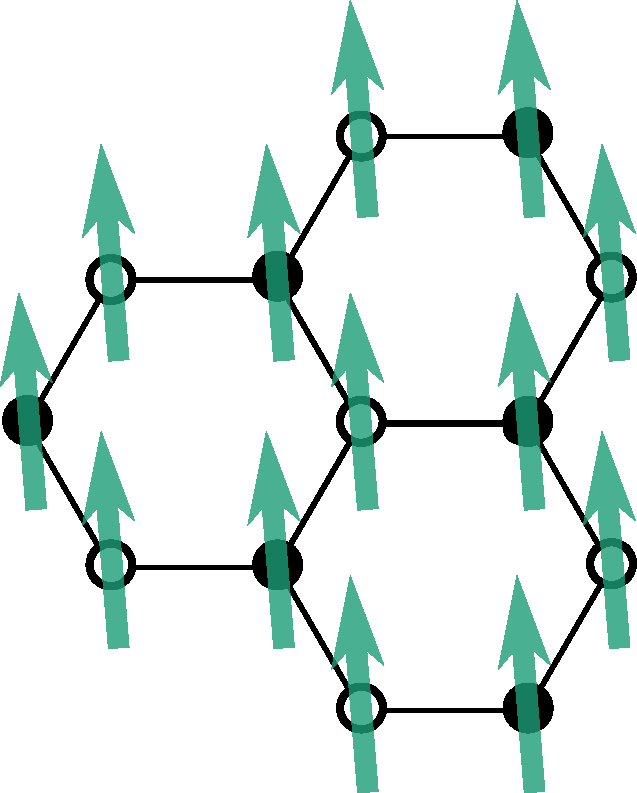
\includegraphics[width=0.2\textwidth]{gfx/hex_ferro}}%
    \hspace{0.05\textwidth}
    \subcaptionbox{N\'eel AFM}{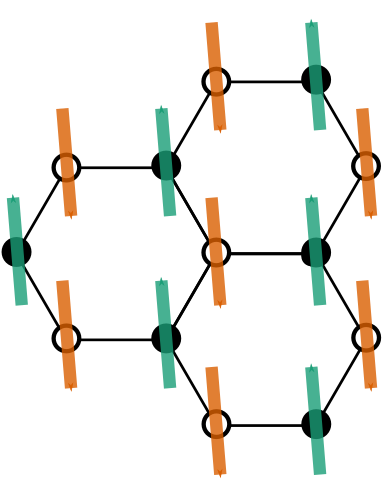
\includegraphics[width=0.2\textwidth]{gfx/hex_AFM_neel}}%
    \hspace{0.05\textwidth}
    \subcaptionbox{Zig-zag AFM}{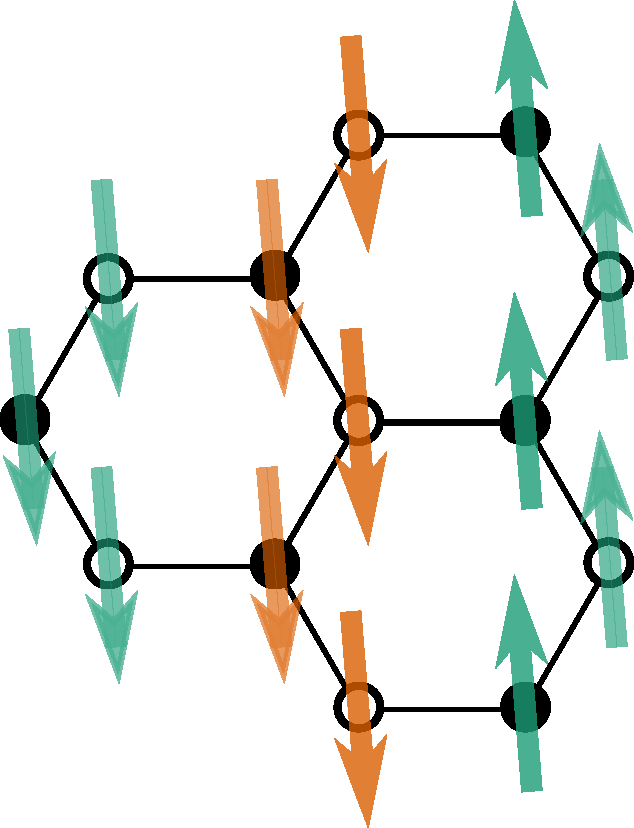
\includegraphics[width=0.2\textwidth]{gfx/hex_AFM_zigzag}}%
    \hspace{0.05\textwidth}
    \subcaptionbox{Stripy AFM}{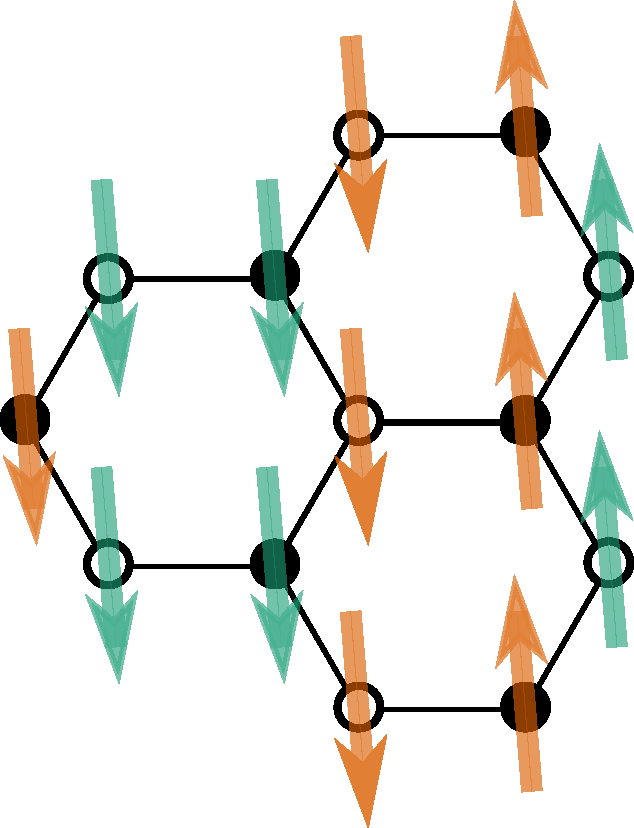
\includegraphics[width=0.2\textwidth]{gfx/hex_AFM_stripy}}%
    \caption{Four magnetic phases commonly found among van-der-Waals magnets.  }
    \label{fig:magnetic_phases}
\end{figure}

Apart from the crystals in Table~\ref{table:crystals}, there is also a large amount of two-dimensional crystals that are neither ferro- or antiferromagnetic. The possibility to induce (anti)ferromagnetism in such a crystal is attractive as it gives access to even a wider range of material parameters. In general one can undertake three ways: (i) doping and defects \cite{gonzalez-herrero_atomic-scale_2016, han_perspectives_2016, ugeda_missing_2010, han_graphene_2014, boukhvalov_sp-electron_2011, boukhvalov_hydrogen_2008, nair_dual_2013}; (ii) magnetic proximity \cite{gonzalez-herrero_atomic-scale_2016, han_perspectives_2016, ugeda_missing_2010, han_graphene_2014}; (iii) strain engineering \cite{shen_strain_2016, chittari_carrier-_2020}.

The first is by chemically doping the crystal with $d$ or $f$ elements (e.g. Mn, Eu, Cr) or by introducing defects. For example, by doping GaAs with Mn atoms, exchange is introduced between local and delocalized spins giving rise to ferromagnetism \cite{dietl_dilute_2014}. Selectively introducing defects on only one sublattice in graphene can also induce weak ferromagnetism -- a consequence of Lieb's theorem \cite{lieb_two_1989, lieb_two_1989-1}. The second approach is by bringing the crystal in vicinity with a (anti)ferromagnetic material. For example one can deposit graphene on top of an insulating ferromagnet such as YIG or EuS to create ferromagnetic graphene \cite{wang_proximity-induced_2015,leutenantsmeyer_proximity_2016}. The third approach makes use of the fact that electronic properties change by means of strain. A compressive strain of $\sim1\%$ in FeSiS$_3$ is predicted \cite{chittari_carrier-_2020} to transition it from a ferromagnetic ground state to a antiferromagnetic ground state. 

Other properties such as spin-orbit coupling \cite{soumyanarayanan_emergent_2016, liu_spin-torque_2011} and magnetocrystalline anisotropy \cite{soumyanarayanan_emergent_2016, dieny_perpendicular_2017} can be tuned or induced as well by placing a magnetic layer on top of a heavy metal layer such as Pt, Ta or W \cite{hellman_interface-induced_2017}. As an example, recently strong current induced spin-orbit torques were measured in a bilayer consisting of Fe$_3$GeTe$_2$ and Pt \cite{wang_current-driven_2019}. 

\subsection{Dirac ferro- and antiferromagnets}
In this Thesis we are interested in the role of conducting electrons in assisting in the manipulation and relaxation of magnetic moments in ferro- and antiferromagnets. Specifically, we study two-dimensional ferro- and antiferromagnets where the conducting electrons have a linear energy dispersion. Such electrons are called Dirac fermions and the system as a whole is referred to as either a Dirac ferro- or antiferromagnet. 

Dirac fermions were first found in graphene \cite{novoselov_electric_2004, novoselov_two-dimensional_2005-1, novoselov_two-dimensional_2005} and soon after in topological insulators \cite{hasan_colloquium_2010, konig_quantum_2008, qi_quantum_2009, cayssol_introduction_2013}. The Dirac ferromagnet that is studied in Chapter~\ref{ch:diffusive} is inspired by a bilayer consisting of a topological insulator and a ferromagnetic insulator. The model can be directly used to describe for example a bilayer consisting of Bi$_2$Te$_3$ or Bi$_2$Se$_3$ and YIG or EuS. 

In Chapters~\ref{ch:summit} and \ref{ch:baglay} a particular antiferromagnet is studied on a honeycomb lattice. Although most of the antiferromagnets presented in Table~\ref{table:crystals} have a honeycomb lattice, the majority are unfortunately non-metallic, or are not in the N\'eel antiferromagnetic phase (illustrated in Fig.~\ref{fig:magnetic_phases}(b)). Recent DFT calculations \cite{chittari_carrier-_2020} predict however a metallic N\'eel antiferromagnetic phase for the following monolayer transition metal trichalgenides: FeSiSe$_3$, FeSiTe$_3$, VGeTe$_3$, MnGeS$_3$, FeGeSe$_3$, FeGeTe$_3$, NiGeSe$_3$, MnSnS$_3$, MnSnS$_3$, MnSnSe$_3$, FeSnSe$_3$, NiSnS$_3$. Experimental realizations of one of these materials could serve as a testing place for our model. 

Furthermore, not every hexagonal metallic N\'eel antiferromagnet can accurately be described with a simple Dirac Hamiltonian. The closest experimentally realized material would be CuMnAs that has a square lattice, but can host Dirac electrons. The results from Chapters~\ref{ch:summit} and \ref{ch:baglay} can at least qualitatively describe the current induced phenomena found in CuMnAs.

Other Dirac antiferromagnets exist as well (e.g. TaCoTe$_2$ \cite{wang_antiferromagnetic_2017}, Zr$_2$Si \cite{shao_zr2si_2018}
, BaFe$_2$As$_2$ and SrFe$_2$As$_2$ \cite{chen_two-dimensional_2017}, EuCd$_2$As$_2$ \cite{ma_emergence_2020}, MnBi$_2$Te$_4$ \cite{swatek_gapless_2020}), but they suffer from symmetry protected gapless states and low exchange energies between localized and conducting electrons. As such, they are unideal when it comes to manipulating the antiferromagnetic order. 

Ideally our model would be directly applied to an antiferromagnetic version of graphene. Though currently non-existent, it has recently been predicted that antiferromagnetism can be induced in graphene by bringing it in proximity with MnPSe$_3$ \cite{hogl_quantum_2020} or by bringing it in double proximity between a layer of Cr$_2$Ge$_2$Te$_6$ and WS$_2$ \cite{zollner_purely_2019}.

\section{Overview of this Thesis}
The general framework of our study revolves around using the $s$--$d$ model to describe the conducting electrons in ferro- and antiferromagnets. By computing the spin-density of these electrons we obtain equations describing the motion and relaxation of magnetic moments. This framework is presented in Chapter~\ref{ch:sdmodel}. The model is applied to a Dirac ferromagnet in Chapter~\ref{ch:diffusive}, which as mentioned above consists of a bilayer of a ferromagnetic insulator and a topological insulator. We find that the unique spin-momentum locking found in topological insulators give rise to a diffusive contribution to the spin-density only in the out-of-plane component. This in turn could lead to more rich and efficient spintronic devices. The remaining chapters are devoted to the study of a hexagonal antiferromagnet. In Chapter~\ref{ch:summit} we develop a numerical method to efficiently calculate torques on magnetizations. This method includes the effect of disorder that, together with spin-orbit interaction and local exchange interactions, forms a microscopic mechanism for the dissipation of magnetic moment to the lattice. Such a microscopic mechanism is often omitted in numerical studies. In Chapter~\ref{ch:baglay}, the same model is studied but solved analytically in a large energy limit. The results are consistent with those in Chapter~\ref{ch:summit}, and are extended by including calculations for various dampings. 

%2D Dirac AFMs
%massless
%TaCoTe2 (https://arxiv.org/pdf/1910.07716.pdf)
%https://journals.aps.org/prb/abstract/10.1103/PhysRevB.95.115138

%Zr2Si %(https://pubs.rsc.org/en/content/articlelanding/2018/cp/c7cp08108a#!divAbstract)

%BaFe2As2 and SrFe2As2 (https://journals.aps.org/prl/abstract/10.1103/PhysRevLett.119.096401)

%https://journals.aps.org/prl/abstract/10.1103/PhysRevLett.118.106402
% "Electric Control of Dirac Quasiparticles by Spin-Orbit Torque in an Antiferromagnet"

%https://onlinelibrary.wiley.com/doi/full/10.1002/adma.201907565?casa_token=pRwIe09TghgAAAAA%3ASLIOXukGo4WJOwC5MNXQmnD4d345pyV76pEKAMWnadsciP7FBVInHvxQPcfZNNZb_0xQY9HZtMxs-_jexw
% "Emergence of Nontrivial Low‐Energy Dirac Fermions in Antiferromagnetic EuCd2As2"

% https://journals.aps.org/prb/abstract/10.1103/PhysRevB.101.161109
% "Gapless Dirac surface states in the antiferromagnetic topological insulator 
% MnBi2Te4"

% honeycomb afm AB
% https://link.springer.com/content/pdf/10.1140/epjb/e2020-100444-8.pdf
% Inorganic materials such as Na2Co2TeO6 [15], BaCo2(AsO2)2 [16], are
% examples of honeycomb lattice spin half antiferromagnets.

% 15. E. Lefancoise et al., Phys. Rev. B 94, 214416 (2016)
% 16. N. Martin, L.-P. Regnault, S. Klimko, J. Phys.: Conf. Ser.
% 340, 012012 (2012)

% zigzag Na2Co2TeO6
% https://journals.aps.org/prb/abstract/10.1103/PhysRevB.95.094424

% Proximity Graphene:
% - graphene + MnPSe3
% "Quantum Anomalous Hall Effects in Graphene from Proximity-Induced Uniform and
% Staggered Spin-Orbit and Exchange Coupling"
% https://journals.aps.org/prl/abstract/10.1103/PhysRevLett.124.136403

% - graphene + Cr2Ge2Te6 and WS2
% "Purely interfacial and highly tunable spin-orbit torque operating field-effect transistor
% in graphene doubly proximitized by two-dimensional magnet Cr2Ge2Te6 and WS2"
% https://arxiv.org/pdf/1910.08072.pdf


% tmdcs adatom doping magnetic proximity
% nature nanotechnology 9 794 (2014)
% prl 104 096804
% nat phys 8 199
% apl mater 4 032401
% science 352 437 

% intrinsic 2d magnets
% 41. N. Samarth, Condensed-matter physics: Magnetism in flatland, Nature 546, 216 (2017). 
% 42. B. Huang, G. Clark, E. Navarro-Moratalla et al., Layer-dependent ferromagnetism in a van-der-Waals crystal down to the monolayer limit, Nature 546, 270 (2017). 
% 43. C. Gong, L Li, Z. Li, et Discovery of intrinsic ferromagnetism in two-dimensional van-der-Waals crystals, Nature 546, 265 (2017). 
% 44. J.-U. Lee, S. Lee, J. H. Ryoo et al., Ising-type magnetic ordering in atomically thin FePS„ Nano Lett. 16, 7433 (2016). 
% 45. W. Xing, Y. Chen, P. M. Odenthal et al., Electric field effect in multilayer Cr2Ge2Te,: A ferromagnetic 2D material, 2D Mater. 4, 024009 (2017). 
% 46. M. Arai, R. Moriya, N. Yabuki, S. Masubuchi, K. Ueno, and T. Machida, Construction of van-der-Waals magnetic tunnel junction using ferromagnetic layered dichalcogenide, Appl. phys. Lett 107, 103107 (2015).

% MoS2 spin valley coupling (vdW material)

% magnetic properties graphene
% https://www.sciencedirect.com/science/article/pii/B9780081021545000059

% "Particularly, carbon-based
% materials are of extreme interest since their structures are generally stable, simple, versatile
% and easy to be modified, which results in easier theoretical magnetism prediction and more
% likely spin induction."

% " Experimentally, creating robust magnetic moments in
% graphene remains very difficult. Approximately, the approaches can be roughly divided into
% three categories: (1) the vacancy approach (creation of the magnetic moments on the basalplane sites by vacancy via ion irradiation), (2) the edge approach (creation of the edge
% magnetic moments at the edge sites by edge-type defects), and (3) the sp3 approach"

% vacancy: lieb's theorem

% "showed the presence of localized electronic states at the zigzag edges (edge states), whereas
% the armchair edge does not exhibit this feature [19,48]. The edge states of ZGNRs extend
% along the edge direction and decay exponentially into the center of the ribbon. As a result
% of the electron-electron interactions, magnetism appears in ZGNRs by ordering the spins
% along the two ribbon edges with ferromagnetic coupling in the same edge, and
% antiferromagnetic coupling between opposite edges [20,49]"

% "A strong synergy between these two fields has been developed over the last couple of years, giving birth to anew field now referred to as 2D spintronics (Figure 1).The goal is to achieve “the best of both worlds” throughthe exploration and exploitation of spin functionality in2D materials. One intuitive advantage of 2D spintronics,over conventional spintronics using traditional magneticmaterials, is to provide a promising opportunity to pushthe relevant devices to the 2D limit that are also gate-tunableand chemical-tunable and mechanically flexible"

% "interface magnetic proximity"

% "More examples beyond graphene have also been demonstrated in 2D transition-metal dichalcogenides ( TMDs) that have 2D layered structures similar to graphene,8,19-28including spin manipulation using spin-valley coupling in 2D-TMDs and the significantly larger spin-orbit torque than conventional heavy metals at ferromagnet/2D-TMDinterface."

% Proc Natl Acad Sci U S A. 2005;102:10451-10453
% wang QH, Kalantar-Zadeh K, Kis A, Coleman JN,
% Strano MS. Electronics and optoelectronics of two-dimensional
% transition metal dichalcogenides. Nat Nanotechnol. 2012;7:
% 699-712.
% Chhowalla M, Shin HS, Eda G, Li W, Loh KP, Zhang H. The
% chemistry of two-dimensional layered transition metal
% dichalcogenide nanosheets. Nat Chem. 2013;5:263-275.
% Radisavljevic B, Radenovic A, Brivio J, Giacometti V, Kis A.
% Single-layer MOS-2 transistors. Nat Nanotechnol. 2011
% Mak KF, Lee C, Hone J, Shan J, Heinz TF. Atomically thin
% MOS : a new direct-gap semiconductor. Phys Rev Lett. 2010;105:
% 136805.
% Xiao D, Liu GB, Feng WX, et al. Coupled spin and valley phys-
% ics in monolayers of MoS2 and other group-VI dichalcogenides.
% Phys Rev Lett.
% Zeng HL, Dai JF, Yao W, Xiao D, Cui X. valley polarization in
% monolayers by optical pumping. Nat Nanotechnol. 2012;7:
% 490-493.
% Butler SZ, Holien SM, Cao LY, et al. Progress, challenges, and
% opportunities in two-dimensional materials beyond graphene.
% ACS Nano.
% Ma YD, Dai Y, Guo M, Niu C, Zhu Y, Huang B. Evidence of the
% existence of magnetism in pristine VX2 monolayers (X S, Se)
% and their strain-induced tunable magnetic properties. ACS Nano.
% Zhang Y, Chang TR, Zhou B, et al. Direct observation of the transition from indirect to direct bandgap in atomically thin epi- taxial MoS2. Nat Nanotechnol. Ugeda MM, Bradley AJ, Zhang Y, et al. Characterization of col- lective ground states in single-layer NbSe2. Nat Phys. 2016; 12: 92-97. Yang LY, Sinitsyn NA, Chen WB, et al. Long-lived nanosecond spin relaxation and spin coherence of electrons in monolayer MOS and WS2. Nat Phys.

% "The first demonstration of 2D-vdW magnets is arguablythe defining moment of 2D spintronics.32,33Unlike most ofthe abovementioned milestone discoveries in graphene andgroup-VI 2D-TMDs where pseudo-spins are involved, 2D-vdW magnets exhibit active carrier spins, just like traditional3d ferromagnets"

% Gong C, Li L, Li ZL, et al. Discovery of intrinsic ferromagnetismin two-dimensional van-der-Waals crystals. Nature. 2017;546:265-269

% Huang B, Clark G, Navarro-Moratalla E, et al. Layer-dependentferromagnetism in a van-der-Waals crystal down to the mono-layer limit. Nature. 2017;546:270-273.

% Castro Neto AH. Charge density wave, superconductivity, andanomalous metallic behavior in 2D transition metaldichalcogenides. Phys Rev Lett. 2001;86:4382-4385.

% "The Mermin-Wagner theorem for many decades has servedas a “rule of thumb” for the understanding of 2D magnetism.55The theorem states that at any nonzero temperature, a long-range magnetic order, be it ferromagnetic or antiferromagnetic,cannot exist in a truly isotropic 2D system, because of its magnon excitation gap being incapable of resisting thermal agitations that collapse the spin ordering. It has been shown that even a small uniaxial magnetic anisotropy can open up a large magnon excitation gap, which in turn lifts the restric-tions imposed by the Mermin-Wagner theorem and results infinite Curie temperatures below which a 2D magnet can practically survive."

% "Transition-metal phosphorus trichalcogenide MPX3(M = Mn, Fe, Co, Ni; X = S, Se) as an emerging group ofvdW-antiferromagnets has fueled much recent theoreticaland experimental efforts."
% Joy PA, Vasudevan S. Magnetism in the layered transition-metalthiophosphates MPS3 (M = Mn, Fe, and Ni). Phys Rev B. 1992;46:5425-5433
% Mayorga-Martinez CC, Sofer Z, Sedmidubský D, Huber Š,Eng AYS, Pumera M. Layered metal thiophosphite materials:magnetic, electrochemical, and electronic properties. ACS ApplMater Interfaces. 2017;9:12563-12573.

% "For instance, antiferromagnetism in CoPS3and NiPS3is of theXY-type for which in the same layer, double-parallel ferromag-netic chains couple antiferromagnetically with each other"

% "ThemagneticstructureofMnPS3consists of a magnetic ioncoupled antiferromagnetically with its nearest neighbors in thelayer, so that their moments are perpendicular to the layerplanes.128,130This is the isotropic Heisenberg-type. In FePS3,the magnetic easy axis also lies perpendicular to the layers.Within a layer, each Fe2+ion is ferromagnetically coupled withtwo of its nearest neighbors and antiferromagnetically with thethird one. However, unlike the XY-type spin orientation, the moments in one plane are antiferromagnetically coupled withneighboring planes, that is, an Ising-type antiferromagnet-ism.124,125,128,130,134,135"

% 124. Lee J-U, Lee S, Ryoo JH, et al. Ising-type magnetic ordering inatomically thin FePS3. Nano Lett. 2016;16:7433-7438.125. Wang X, Du K, Fredrik Liu YY, et al. Raman spectroscopy ofatomically thin two-dimensional magnetic iron phosphorus trisul-fide (FePS3) crystals. 2D Mater. 2016;3:031009.

% 128. Joy PA, Vasudevan S. Magnetism in the layered transition-metalthiophosphates MPS3 (M = Mn, Fe, and Ni). Phys Rev B. 1992;46:5425-5433.

% 130 Bernasconi M, Marra GL, Benedek G, et al. Lattice dynamics oflayered MP3(M = Mn, Fe, Ni, Zn; X = S, Se) compounds. PhysRev B. 1988;38:12089-12099.

% 134 Rule KC, Kennedy SJ, Goossens DJ, Mulders AM, Hicks TJ.Contrasting antiferromagnetic order between FePS3and MnPS3.Appl Phys A. 2002;74:s811-s813.

% 135 K-z D, Wang X-z, Liu Y, et al. Weak van-der-Waals stacking,wide-range band gap, and Raman study on ultrathin layers of metalphosphorus trichalcogenides. ACS Nano. 2016;10:1738-1743.

% Fe3GeTe2 (https://advances.sciencemag.org/content/5/8/eaaw8904) on Pt and Pa
% tunable curie temperature, conducting, large spin orbit.




